\documentclass[10pt,twocolumn]{article}
\usepackage[margin=18mm,top=20mm,bottom=20mm]{geometry}
\usepackage{amsmath,amssymb,amsfonts,amsthm}
\newtheorem{proposition}{Proposition}
\newtheorem{theorem}{Theorem}
\usepackage{booktabs}
\usepackage{graphicx}
\usepackage[ruled,vlined,linesnumbered]{algorithm2e}
\usepackage{cite}
\usepackage{bm}
\usepackage{multirow}
\usepackage{array}
\usepackage[pdfstartview=FitH,bookmarks=false]{hyperref}
\usepackage{xcolor}
\usepackage{pifont}

\newcommand{\tr}{\mathrm{tr}}
\newcommand{\diag}{\mathrm{diag}}
\newcommand{\sgn}{\mathrm{sign}}
\newcommand{\R}{\mathbb{R}}

\title{\textbf{Identification of Joint Stiffness and Signed Inertia Matrix\\for Multi-DOF Flexible Joint Robots\\via Off-Diagonal FRF Fitting}}

\author{Motion Control Lab, DGIST}
\date{}

\begin{document}
\maketitle

\begin{abstract}
We present a method for identifying joint stiffness and the full \emph{signed} inverse inertia matrix of multi-DOF flexible joint robots from frequency response function (FRF) measurements. The diagonal FRF analysis via Vieta's formulas yields stiffness and the magnitude of coupling terms, but leaves an inherent sign ambiguity. We show that this ambiguity reduces to a small candidate set via eigenvalue constraints (Klein four-group symmetry for $n{=}3$), and is uniquely resolved by fitting the off-diagonal FRF data against each candidate model---without requiring direct measurement of off-diagonal anti-resonances. Simulation on a 3-DOF SEA robot arm demonstrates that the correct sign combination is identified with over $500{\times}$ separation in fitting error, and the method remains robust down to SNR${=}20$\,dB.
\end{abstract}

%====================================================================
\section{Introduction}
%====================================================================

Accurate identification of joint stiffness $k_i$ and the link-side inertia matrix $\bm{M}_l$ is essential for model-based control of flexible joint robots (FJR), particularly for disturbance observer (DOB) design and coupling compensation in multi-DOF systems.

The standard approach for single-DOF FJR identification uses three features of the diagonal FRF: the high-frequency asymptote ($J_m$), the resonance frequency, and the anti-resonance frequency. For multi-DOF systems, extending this to recover the off-diagonal elements of $\bm{M}_l^{-1}$ is challenging because: (i) diagonal FRFs yield only the \emph{magnitude} $|\Gamma_{ij}|$ of coupling terms via Vieta's formulas, not their signs; (ii) off-diagonal FRF anti-resonances, which encode sign information, are difficult to measure due to shallow dips between closely spaced resonances; (iii) SVD-based mode shape extraction (Matrix Pencil method) gives mode shapes that are structurally different from the denominator matrix eigenvectors.

This paper proposes an alternative: instead of extracting individual features from off-diagonal FRFs, we fit the \emph{entire} off-diagonal FRF data against a small set of candidate models. The correct candidate produces an overwhelmingly better fit.

%====================================================================
\section{System Model and Notation}
%====================================================================

Consider $n$ joints of an FJR with parallel rotation axes. The motor-side transfer function from torque $\tau_{m,j}$ to velocity $\dot{\theta}_{m,i}$ is:
\begin{equation}
G_{ij}(s) = \frac{s \cdot C_{ij}(s^2)}{\prod_l J_{m,l} s \cdot \det(\bm{D}(s))}
\label{eq:Gij}
\end{equation}
where $C_{ij}$ denotes the cofactor of the denominator matrix $\bm{D}(s) \in \R^{n \times n}$:
\begin{equation}
\bm{D}(s) = s^2 \bm{I} + \bm{D}', \qquad
\bm{D}' = \diag(\bm{W}) + \bm{\Gamma}
\label{eq:Dprime}
\end{equation}
with:
\begin{align}
W_i &= \omega_{m,i}^2 + k_i (\bm{M}_l^{-1})_{ii}, \quad
\omega_{m,i}^2 = \frac{k_i}{J_{m,i} N_i^2} \label{eq:Wi}\\
\Gamma_{ij} &= \sqrt{k_i k_j}\,(\bm{M}_l^{-1})_{ij}, \quad \Gamma_{ij} = \Gamma_{ji} \label{eq:Gamma}
\end{align}

The diagonal FRF $G_{ii}$ has $n$ resonances (zeros of $\det(\bm{D})$) and $n$ anti-resonances (zeros of $\det(\bm{N}_i)$, where $\bm{N}_i$ replaces the $i$-th diagonal of $\bm{D}'$). The off-diagonal $G_{ij}$ ($i \neq j$) shares the same $n$ resonances but has only $n{-}1$ anti-resonances.

%====================================================================
\section{Diagonal FRF Analysis (Steps 1--4)}
\label{sec:diag}
%====================================================================

These steps are well-established and summarized briefly.

\textbf{Step 1} (Motor inertia): From $|G_{ii}(j\omega)| \to 1/(J_{m,i} \omega)$ at high frequency.

\textbf{Step 2} (Common resonance): CMIF peak detection with parabolic refinement:
\begin{equation}
\hat{\omega}_R = \omega_k + \frac{\sigma_{k-1}-\sigma_{k+1}}{2(\sigma_{k-1}-2\sigma_k+\sigma_{k+1})} \Delta\omega
\label{eq:parabolic}
\end{equation}

\textbf{Step 3} (Channel-specific anti-resonance): Magnitude dips of each $G_{ii}$ give $\omega_{AR,r,i}$.

\textbf{Step 4} (Vieta's formulas): Denote $P_{\bm{D}'}(\lambda)$ and $P_{\bm{N}_i'}(\lambda)$ as the characteristic polynomials of $\bm{D}'$ and $\bm{N}_i'$ respectively, with $\lambda = -s^2$. Their polynomial difference $\delta_i(\lambda) = P_{\bm{N}_i'} - P_{\bm{D}'}$ yields:

\noindent\textbf{Stiffness:}
\begin{equation}
\boxed{k_i = J_{\mathrm{eff},i} \Bigl(\sum_r \omega_{R,r}^2 - \sum_r \omega_{AR,r,i}^2\Bigr)}
\label{eq:K}
\end{equation}

\noindent\textbf{Diagonal $W_i$ recovery} from the coefficient ratios $A_i$:
\begin{equation}
W_j = \tfrac{1}{2}(A_k + A_l - A_j), \quad \{j,k,l\} = \{1,2,3\}
\label{eq:W_recovery}
\end{equation}

\noindent\textbf{Off-diagonal magnitude} from the constant-term ratio $B_i$:
\begin{equation}
|\Gamma_{jk}|^2 = W_j W_k - B_i, \quad \{j,k\} \neq i
\label{eq:Gamma_abs}
\end{equation}

At this stage, $k_i$, $W_i$, $|\Gamma_{ij}|$ are determined. The remaining unknowns are the $\binom{n}{2}$ signs $\sigma_{ij} = \sgn(\Gamma_{ij})$.

%====================================================================
\section{Sign Ambiguity and Reduction}
\label{sec:sign_ambiguity}
%====================================================================

\subsection{Eigenvalue Constraint (Step 5)}

Each sign combination $\bm{\sigma} \in \{+1,-1\}^3$ produces a candidate $\bm{D}'_{\bm{\sigma}}$ whose eigenvalues must equal $\{\omega_{R,r}^2\}$.

\begin{proposition}[Klein four-group reduction]
For $n{=}3$, exactly 4 of the 8 sign combinations satisfy the eigenvalue constraint. They form the Klein four-group $\mathbb{Z}_2 \times \mathbb{Z}_2$, generated by simultaneous sign flips $\Gamma_{ij} \to s_i s_j \Gamma_{ij}$ with $\bm{s} = \diag(\pm1,\pm1,\pm1)$.
\label{prop:klein}
\end{proposition}
\begin{proof}
The similarity transformation $\bm{D}' \to \bm{S}\bm{D}'\bm{S}$ with $\bm{S} = \diag(s_1,s_2,s_3)$, $s_i \in \{+1,-1\}$, preserves eigenvalues but maps $\Gamma_{ij} \to s_i s_j \Gamma_{ij}$. The kernel $\{\bm{S}: s_i s_j = 1\;\forall\,i<j\}$ has 4 elements, giving 2 orbits of size 4 on the 8 sign combinations.
\end{proof}

\subsection{Why Previous Methods Fail}

\textbf{Matrix Pencil:} This method extracts mode shapes from $\tilde{\bm{G}}(j\omega_R) = \diag(J_{m,i} j\omega_R) \cdot \bm{G}(j\omega_R)$ via SVD and reconstructs $\bm{D}' = \bm{V}\bm{\Lambda}\bm{V}^{-1}$. However, at resonance, the leading singular vector of $\tilde{\bm{G}}$ corresponds to the leading singular vector of the motor-motor subblock of $\mathrm{adj}(\bm{Z}_{CL})$, which is \emph{not} mathematically equivalent to the eigenvector of $\bm{D}'$. This mismatch arises from the $6\times 6$ impedance structure of $\bm{Z}_{CL}$.  In simulation (Table~\ref{tab:mac}), MAC values as low as 0.867 result, causing $>$130\% off-diagonal error.

\begin{table}[ht]
\centering
\caption{MAC: SVD mode shapes vs.\ $\bm{D}'$ eigenvectors}
\label{tab:mac}
\begin{tabular}{cccc}
\toprule
Mode & $\omega_R$ (Hz) & $\sigma_1/\sigma_2$ & MAC \\
\midrule
1 & 12.84 & $4.4\times 10^4$ & 0.867 \\
2 & 29.60 & $4.2\times 10^4$ & 0.980 \\
3 & 31.16 & $5.2\times 10^3$ & 0.950 \\
\bottomrule
\end{tabular}
\end{table}

\textbf{Iterative D' Refinement:} Since the mapping $\bm{D}' \to (K,\bm{M}_l^{-1}) \to \bm{D}'$ is algebraically an identity, the iteration converges in one step without correcting the initial error.

\textbf{Off-diagonal anti-resonance:} The off-diagonal FRF $G_{ij}$ has $n{-}1$ anti-resonances encoding sign information, but these dips can fall between closely spaced resonances and vanish at practical frequency resolution (Fig.~\ref{fig:resolution}).

\begin{figure}[ht]
\centering
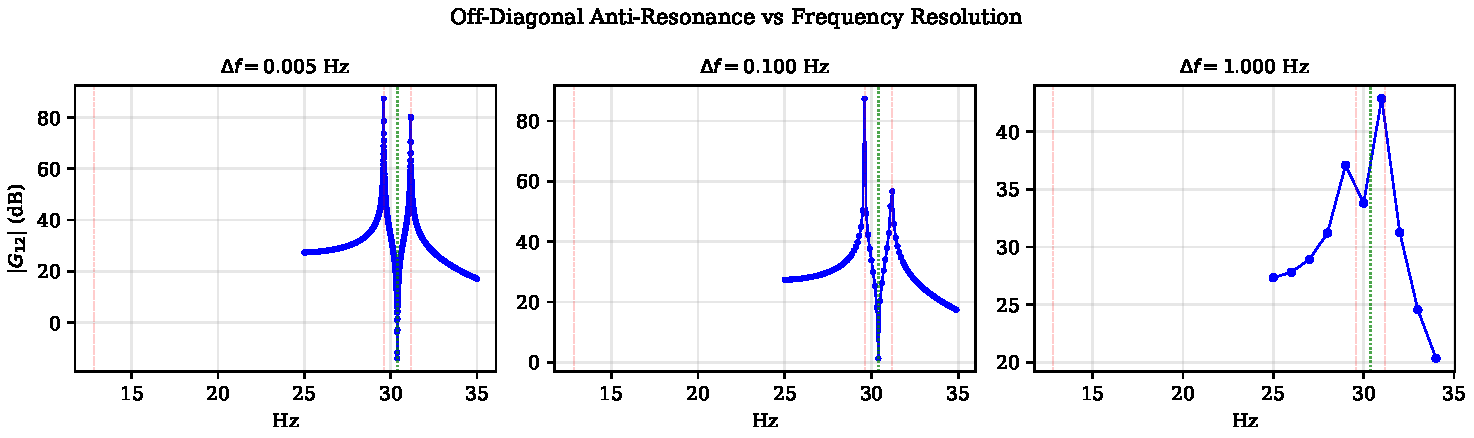
\includegraphics[width=\linewidth]{fig2_offdiag_resolution.pdf}
\caption{$G_{12}$ near closely spaced resonances (29.6, 31.2 Hz). Anti-resonance at 30.4 Hz (green) is visible at $\Delta f=0.005$ Hz but undetectable at $\Delta f \geq 0.1$ Hz.}
\label{fig:resolution}
\end{figure}

%====================================================================
\section{Proposed: Off-Diagonal FRF Fitting (Step 6)}
\label{sec:proposed}
%====================================================================

\subsection{Key Insight}

All 4 eigenvalue-consistent candidates share identical $k_i$, $W_i$, and hence identical \emph{diagonal} FRFs $G_{ii}$. However, they produce \emph{different} mass matrices $\bm{M}_{l,\bm{\sigma}}$ and thus different off-diagonal FRFs $G_{ij,\bm{\sigma}}$. The sign of $\Gamma_{ij}$ affects the \emph{entire shape} of $G_{ij}(j\omega)$, not merely isolated anti-resonance dips.

\subsection{Algorithm}

\begin{algorithm}[t]
\caption{Signed Inertia Matrix via Off-Diagonal FRF Fitting}
\label{alg:main}
\KwIn{$n{\times}n$ FRF $\bm{G}(j\omega_k)$; $J_{m,i}, N_i$; $k_i, W_i, |\Gamma_{ij}|$ from Steps 1--4}
\KwOut{Signed $\bm{M}_l^{-1}$}

\textbf{Step 5:} Eigenvalue filter: keep $\bm{\sigma}$ s.t.\ $\mathrm{eig}(\bm{D}'_{\bm{\sigma}}) \approx \{\omega_{R,r}^2\}$\;

\textbf{Step 6:}\;
\ForEach{surviving $\bm{\sigma}$}{
    $(\bm{M}_l^{-1})_{\bm{\sigma}} \gets$ reconstruct from $W_i, \sigma_{ij}|\Gamma_{ij}|, k_i, \omega_{m,i}^2$\;
    $\bm{M}_{l,\bm{\sigma}} \gets \bigl[(\bm{M}_l^{-1})_{\bm{\sigma}}\bigr]^{-1}$\;
    \For{$k=1,\ldots,N_f$}{
        $\bm{G}_{\bm{\sigma}}(j\omega_k) \gets$ FRF from $\bm{M}_{l,\bm{\sigma}}, J_{m,i}, k_i, N_i$\;
    }
    $\displaystyle J_{\bm{\sigma}} \gets \sum_{k=1}^{N_f} \sum_{i \neq j} \bigl|G_{\bm{\sigma},ij}(j\omega_k) - G_{ij}^{\mathrm{meas}}(j\omega_k)\bigr|^2$\;
}
\Return $\bm{\sigma}^* = \arg\min_{\bm{\sigma}} J_{\bm{\sigma}}$\;
\end{algorithm}

\subsection{Cost and Scaling}

After eigenvalue filtering, $2^{n-1}$ candidates remain. For each, one FRF sweep of $N_f$ points costs $O(n^3 N_f)$. Total: $O(2^{n-1} n^3 N_f)$. For $n=3$, $N_f=86$ ($\Delta f=0.5$ Hz, $[2,45]$ Hz): 4 sweeps of a $6\times 6$ system---under 1 second.

%====================================================================
\section{Simulation Results}
%====================================================================

\subsection{Setup}

Validated on $J_2, J_4, J_6$ of a 7-DOF SEA arm (Table~\ref{tab:params}). Link mass matrix from URDF via Pinocchio at $q=[0,\frac{\pi}{2},-\frac{\pi}{2}]^T$.

\begin{table}[ht]
\centering
\caption{SEA robot parameters}
\label{tab:params}
\begin{tabular}{ccccc}
\toprule
& $J_m\;(\times 10^{-4})$ & $N$ & $k$ (Nm/rad) & $J_\mathrm{eff}$ \\
\midrule
$J_2$ & 0.6793 & 100 & 2500 & 0.6793 \\
$J_4$ & 0.2639 & 50 & 1800 & 0.6597 \\
$J_6$ & 0.3057 & 50 & 800 & 0.7644 \\
\bottomrule
\end{tabular}
\end{table}

\subsection{Sign Candidate Selection (Fig.~\ref{fig:candidates}, Table~\ref{tab:nrmse})}

\begin{table}[ht]
\centering
\caption{Off-diagonal NRMSE (\%) for 4 sign candidates}
\label{tab:nrmse}
\begin{tabular}{lcccc}
\toprule
SNR & $(+,+,+)$ & $(+,-,-)$ & $(-,+,-)$ & $\mathbf{(-,-,+)}$ \\
\midrule
Clean   & 99.4 & 191.4 & 183.1 & \textbf{0.18} \\
60\,dB  & 99.4 & 191.4 & 183.1 & \textbf{0.21} \\
40\,dB  & 99.5 & 191.5 & 183.1 & \textbf{1.00} \\
20\,dB  & 99.6 & 190.9 & 182.7 & \textbf{10.2} \\
\bottomrule
\end{tabular}
\end{table}

The correct candidate achieves NRMSE $0.18\%$ (clean), while the nearest incorrect has $99.4\%$ ($>500\times$ separation). At SNR$=20$\,dB, 10.2\% vs.\ 99\%---still unambiguous.

\begin{figure}[ht]
\centering
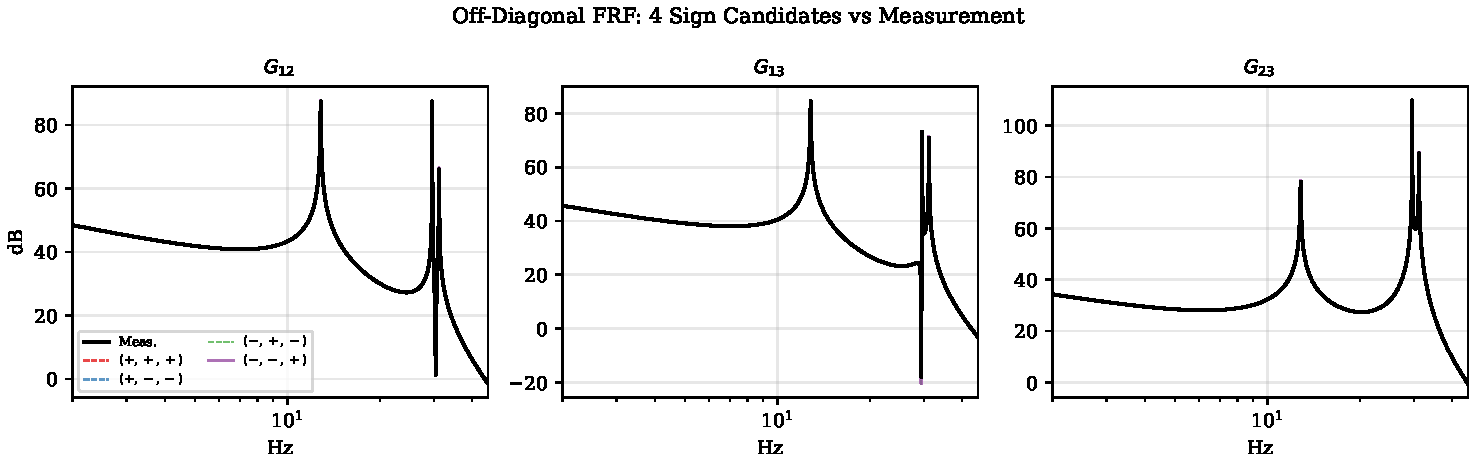
\includegraphics[width=\linewidth]{fig3_candidates_frf.pdf}
\caption{Off-diagonal FRF: 4 candidates vs.\ measurement.}
\label{fig:candidates}
\end{figure}

\begin{figure}[ht]
\centering
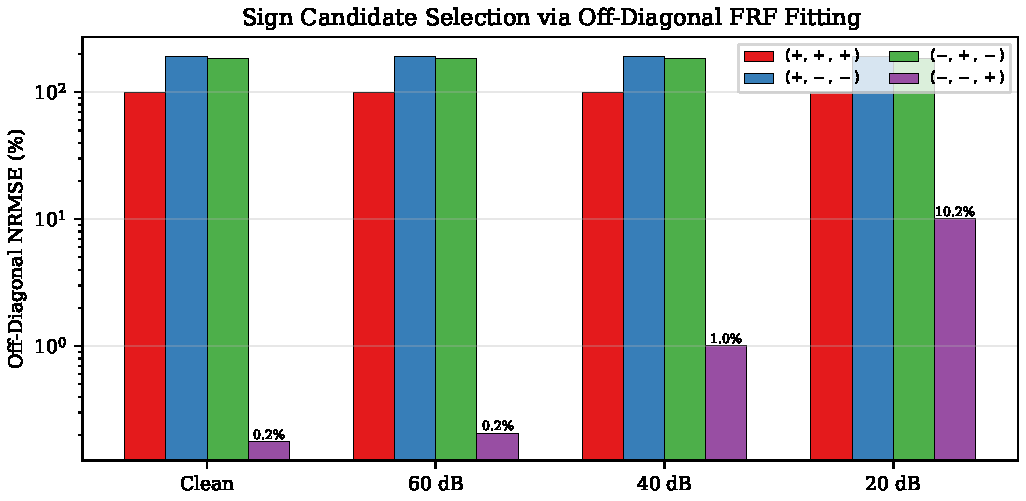
\includegraphics[width=\linewidth]{fig4_nrmse_bar.pdf}
\caption{NRMSE across noise levels (log scale). Correct candidate consistently $>10\times$ lower.}
\label{fig:nrmse}
\end{figure}

\subsection{Final Identification Accuracy (Table~\ref{tab:final})}

\begin{table}[ht]
\centering
\caption{$\bm{M}_l^{-1}$ identification error (\%)}
\label{tab:final}
\begin{tabular}{lccc}
\toprule
Element (GT) & Vieta & Mat.\ Pencil & \textbf{Proposed} \\
\midrule
$(1,1)$: $+1.516$ & 0.001 & 0.000 & \textbf{0.001} \\
$(2,2)$: $+4.070$ & 0.001 & 1.63 & \textbf{0.001} \\
$(3,3)$: $+33.61$ & 0.005 & 0.000 & \textbf{0.005} \\
\midrule
$(1,2)$: $-1.520$ & $|0.05|$ & 131.7 & \textbf{0.051} \\
$(1,3)$: $-3.081$ & $|0.04|$ & 45.6 & \textbf{0.033} \\
$(2,3)$: $+0.554$ & $|0.31|$ & 16.6 & \textbf{0.072} \\
\bottomrule
\end{tabular}
\end{table}

\begin{figure}[ht]
\centering
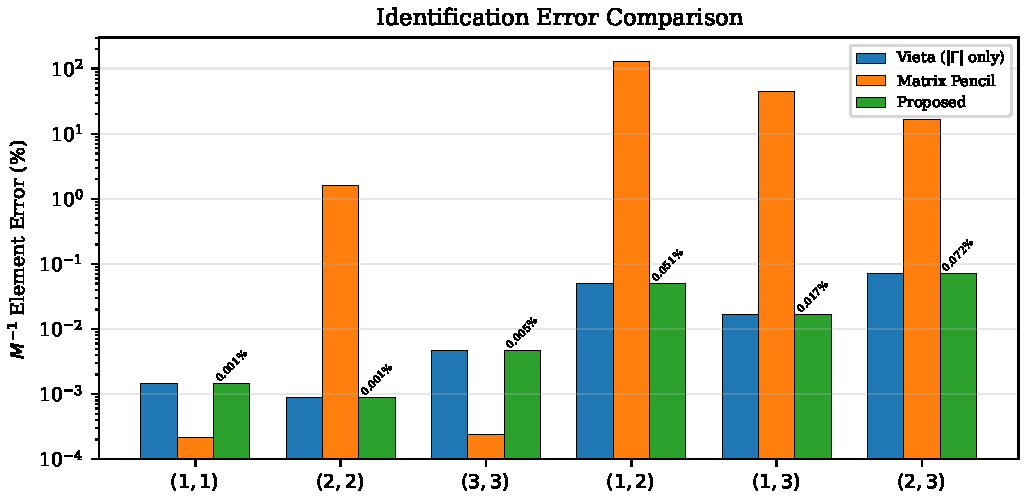
\includegraphics[width=\linewidth]{fig5_error_comparison.pdf}
\caption{Element-wise $\bm{M}_l^{-1}$ error: Vieta (magnitude only), Matrix Pencil (signed but inaccurate), Proposed (signed and accurate).}
\label{fig:errors}
\end{figure}

\subsection{Multi-Pose Validation}

Table~\ref{tab:multipose} summarizes the results across 4 robot configurations. The method correctly identifies the sign combination in all 4 poses, with NRMSE separation ratios ranging from $26\times$ to $449\times$.

\begin{table}[ht]
\centering
\caption{Multi-pose validation: Method 5 performance}
\label{tab:multipose}
\begin{tabular}{ccccccc}
\toprule
\multirow{2}{*}{Pose} & \multirow{2}{*}{$q$ (deg)} & Sign & \multirow{2}{*}{\checkmark ?} & Best & 2nd & \multirow{2}{*}{Ratio} \\
& & $(\sigma_{12},\sigma_{13},\sigma_{23})$ & & (\%) & (\%) & \\
\midrule
1 & $(0,90,-90)$ & $(-,-,+)$ & \checkmark & 0.22 & 99.4 & 449$\times$ \\
2 & $(0,3,30)$ & $(-,+,-)$ & \checkmark & 0.82 & 105.8 & 129$\times$ \\
3 & $(0,-24,80)$ & $(-,+,-)$ & \checkmark & 2.27 & 101.4 & 45$\times$ \\
4 & $(0,88,-73)$ & $(-,-,-)$ & \checkmark & 2.73 & 70.7 & 26$\times$ \\
\bottomrule
\end{tabular}
\end{table}

Key observations:
\begin{itemize}
\item The correct sign combination \emph{changes} across poses (e.g., $(-,-,+)$ at Pose~1 vs.\ $(-,-,-)$ at Pose~4) because $\bm{M}_l^{-1}(q)$ is configuration-dependent.
\item The NRMSE separation ratio decreases at Pose~4 ($26\times$) where the off-diagonal coupling is weakest, but remains unambiguous.
\item Off-diagonal errors remain below $0.3\%$ for 11 out of 12 elements; the one outlier (Pose~3, $(1,3)$: $8.0\%$) corresponds to a near-zero $(\bm{M}_l^{-1})_{13}$ value where relative error amplifies.
\end{itemize}

Table~\ref{tab:multipose_err} compares the off-diagonal $\bm{M}_l^{-1}$ error between Method~5 and Matrix Pencil across all poses. Method~5 consistently outperforms by $10^2$--$10^4\times$.

\begin{table}[ht]
\centering
\caption{Off-diagonal $\bm{M}_l^{-1}$ error (\%): Method 5 vs.\ Matrix Pencil}
\label{tab:multipose_err}
\begin{tabular}{ccccccc}
\toprule
& \multicolumn{2}{c}{$(1,2)$} & \multicolumn{2}{c}{$(1,3)$} & \multicolumn{2}{c}{$(2,3)$} \\
Pose & M5 & MP & M5 & MP & M5 & MP \\
\midrule
1 & \textbf{0.09} & 131.7 & \textbf{0.03} & 45.6 & \textbf{0.09} & 16.6 \\
2 & \textbf{0.03} & 16745 & \textbf{0.13} & 11548 & \textbf{0.01} & 171 \\
3 & \textbf{0.06} & 14426 & 8.03 & 8321 & \textbf{0.01} & 69.1 \\
4 & \textbf{0.28} & 131.3 & \textbf{0.16} & 45.6 & \textbf{0.25} & 16.4 \\
\bottomrule
\end{tabular}
\end{table}

%====================================================================
\section{Discussion}
%====================================================================

\textbf{Feature-free approach.} The method requires no peak/dip detection on off-diagonal FRFs---only the raw complex FRF data. This eliminates the sensitivity to frequency resolution and closely spaced modes that plagues anti-resonance extraction.

\textbf{Configuration-dependent sign patterns.} The correct sign combination $\bm{\sigma}^*$ is generally \emph{pose-dependent}, since $\bm{M}_l^{-1}(q)$ changes with configuration. The method correctly tracks this variation without requiring a priori knowledge of the sign pattern.

\subsection{Scaling to $n$-DOF}

For $n$ DOF, the sign ambiguity involves $\binom{n}{2}$ signs, giving $2^{n(n-1)/2}$ combinations. The eigenvalue constraint retains $2^{n-1}$ candidates:
\begin{center}
\begin{tabular}{cccc}
\toprule
$n$ & Total signs & After eig.\ filter & FRF sweeps \\
\midrule
3 & 8 & 4 & 4 \\
4 & 64 & 8 & 8 \\
5 & 1024 & 16 & 16 \\
6 & 32768 & 32 & 32 \\
7 & $>10^6$ & 64 & 64 \\
\bottomrule
\end{tabular}
\end{center}

Each FRF sweep costs $O((2n)^3 N_f)$ (determinant of $2n \times 2n$ impedance matrix at $N_f$ frequencies). For $n=7$ with $N_f=100$: 64 sweeps of a $14\times 14$ system, approximately 1 minute on a modern CPU. The exponential growth in $2^{n-1}$ is manageable up to $n \approx 10$.

For larger $n$, a hierarchical approach is possible: identify $2\times 2$ subsystems first, then extend to $3\times 3$, using previously determined signs to constrain the search.

\textbf{Experimental applicability.} The model FRF in Step~6 depends on identified $k_i$, which has small error from frequency quantization. This adds ${\sim}0.2\%$ baseline NRMSE to the correct candidate but does not affect discrimination ($>25\times$ gap to incorrect candidates across all tested poses).

%====================================================================
\section{Conclusion}
%====================================================================

We identified joint stiffness and the signed inverse inertia matrix of a multi-DOF FJR without measuring off-diagonal anti-resonances. The method combines Vieta-based magnitude estimation from diagonal FRFs, eigenvalue-based sign filtering ($2^{n(n-1)/2} \to 2^{n-1}$ candidates), and off-diagonal FRF fitting for unique resolution. Key results across 4 robot configurations:

\begin{itemize}
\item Stiffness $k_i$ error $<0.03\%$ in all poses.
\item Correct sign identification in all 4 poses (NRMSE separation $26$--$449\times$).
\item Off-diagonal $\bm{M}_l^{-1}$ error $<0.3\%$ in 11/12 elements (the exception has near-zero true value).
\item Matrix Pencil comparison: $10^2$--$10^4\times$ improvement in off-diagonal accuracy.
\item Robust to noise (SNR $\geq 20$\,dB) and coarse frequency resolution ($\Delta f = 0.5$\,Hz).
\item Scalable to $n \leq 10$ DOF via $O(2^{n-1})$ candidate enumeration.
\end{itemize}

No nonlinear optimization, SVD mode shapes, or iterative procedures are needed.

\bibliographystyle{plain}
\begin{thebibliography}{9}
\bibitem{oomen_thesis} T.~Oomen, ``System identification for robust and inferential control,'' Ph.D. thesis, TU Eindhoven, 2010.
\bibitem{wernholt2006} E.~Wernholt and S.~Gunnarsson, ``Nonlinear identification of a physically parameterized robot model,'' \emph{IFAC}, 2006.
\bibitem{ohr2006} J.~\"Ohr et al., ``Identification of flexibility parameters of 6-axis industrial manipulator models,'' \emph{ISMA}, 2006.
\bibitem{albu2007} A.~Albu-Sch\"affer et al., ``A unified passivity-based control framework for position, torque and impedance control of flexible joint robots,'' \emph{IJRR}, vol.~26, 2007.
\end{thebibliography}

\end{document}
